%\documentclass[main.tex]{subfiles}
%\begin{document}
\chapter{Introduction}
%This is better, but by framing it as having your parents visit, you transform the problem such that it wouldn't be safe to explore. (Rather wait until your parents, and then try out the unknown example). The goal in a bandit task is cumulative reward, so one trial with a bad outcome isn't so bad if you learn something valuable. You're making it sem as if it is the last trial, so it would only make sense to exploit! Also, why not choose 4 coffee shops since we use a 4-armed bandit? Not a big deal if you've already invested the time in the figures though.
Imagine you just moved to a new city for a new job, your parents plan a visit and want to go to a coffee shop with you. You have three coffee shops nearby (see Figure \ref{fig:Coffe_Example}). You have only tried one of them before and have absolutely no clue about the quality of the other two shops. Where will you go? Will you exploit your knowledge about the one coffee shop or will you discover one of the other coffee shops?
Everyone encounters this kind of problem on a regular basis in different kinds of settings and with different constraints, like looking for a new flat, or finding a partner or just deciding which kind of noodle one buys. 
Each time we face such a problem, we are encounter a dilemma about whether we try something new or if we stay with what we already know is pretty good. 
%You need to motivate why this coffee problem is important for cognitive science. Isn't there already a simple solution? Why should the reader care?
This is better known as the exploration-exploitation dilemma. How do you balance between \textit{exploiting} your current knowledge (e.g., going to the coffee shop you know) to acquire immediate rewards, compared to expanding your knowledge by \textit{exploring} (e.g., trying a new coffee shop), which can reduce the uncertainty about the environment.
Gaining new information about the environment makes you better equipped to make future decisions (e.g., what coffee quality you get from which coffee shop). By expanding your knowledge you might even find coffee shops that offer better coffee than the one you already know. By exploiting your current knowledge, you accumulate the best reward you can get at the moment, e.g. you would go to the same coffee place again and enjoy the best coffee currently known to you. 


\begin{figure}
    \centering
    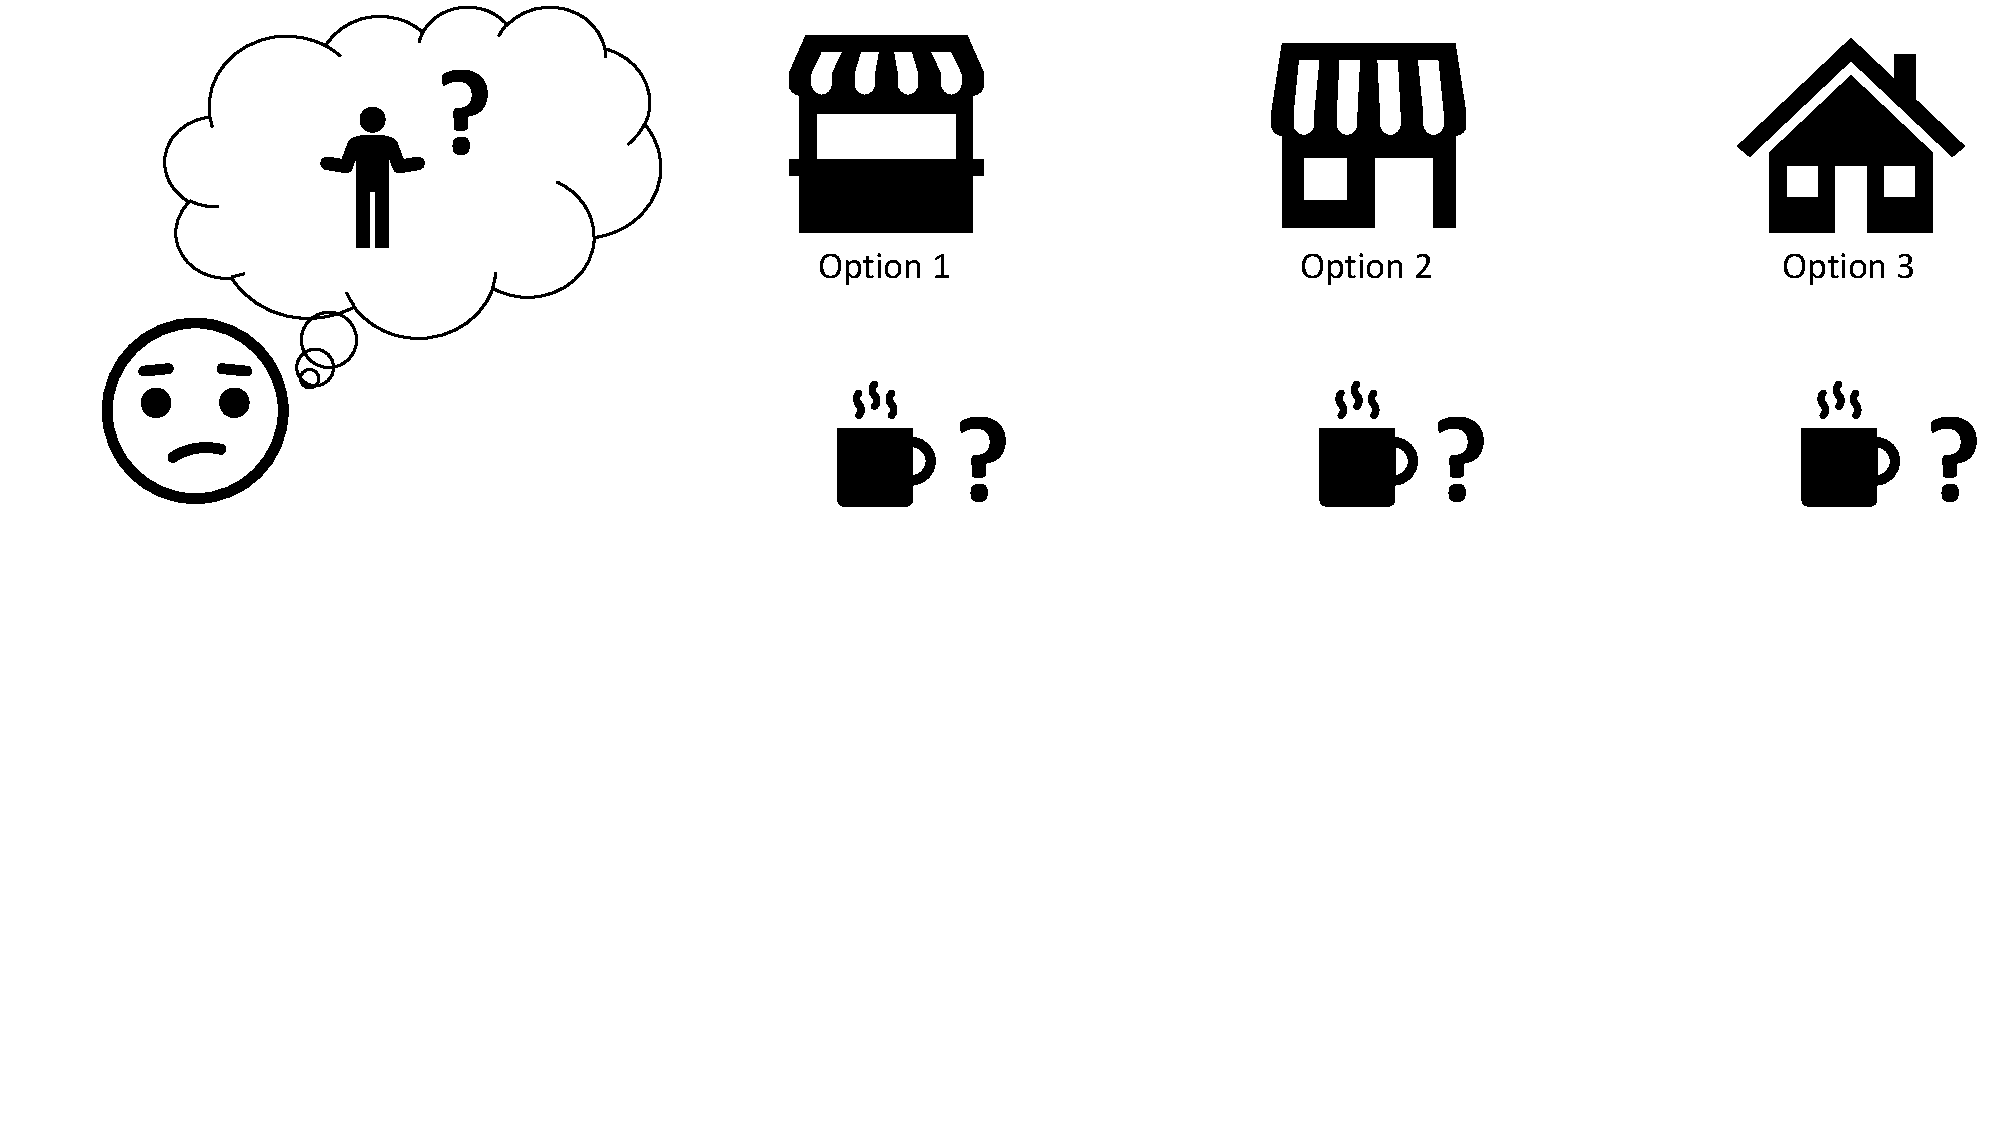
\includegraphics[width=1\textwidth]{Plots/CoffeExample.pdf}
    \vspace{-4cm}
    \caption[Coffee Shop Example]{How to choose a coffee shop. You are completely new in a city and you have multiple options, you do not know anything about the coffee from the different options.}
    \label{fig:Coffe_Example}
\end{figure}


%Why does it play a crucial role? Why is machine learning and AI interested in this coffee problem?
The exploration--exploitation dilemma plays a crucial role in the reinforcement learning (RL) framework \citep{sutton2018reinforcement}, which provides computational solutions to problems where learning occurs through interactions with an environment.
%Here fill in why it plays a crucial role -- needs to be revisited something in this direction
The dilemma lives by interacting with the different options given by the environment and by this exploration or exploitation we gain more knowledge about the environment, we learn which options can be avoided or which should be revisited. This interaction provides the basis for learning associations and rewards, which is what RL is concerned with: learning through interaction. 
%not sure where to put this but I would probbaly phrase the answers to the the questins about why these two diciplies ar einterested in it
Machine learning is concerned with the task that a computer learns from an experience and is then able to perform a task. RL is one of three main learning approaches used in machine learning. 
Artificial Intelligence is concerned with mimicing cognitive abilities like learning through interaction, therefore building a computational model that explains how we solve our coffee problem can be used to mimic the exact same process. 
Modern approaches to RL used in machine learning \citep{sutton2018reinforcement} and artificial intelligence \citep{sutton2018reinforcement, russell2016artificial} are based on psychological models of associative learning \citep{bush1951model,rescorla1972theory,dayan2000learning,sutton2018reinforcement}, which in turn can be traced back to early research on trial and error learning in animals \citep{thorndike1927law, skinner1963operant}.

 
This chapter is structured as follows. %I originally thought this was the structure for the whole thesis, so I added this clarification

To discover how the coffee problem and other instances of the dilemma can be solved, this thesis begins with a history of reinforcement learning, starting with early psychological theories of classical and operant conditioning. %Start with the broader theoretical question, and lean a little less on the coffee example here. It's ok to mention it, but you also need to connect it to the bigger picture of cognition--> why is it hard to behave intelligently when balancing between acquiring immediate rewards and acquiring information?
These theories provide the inspiration for models of associative learning, which are the computational origins of modern reinforcement learning. We can distinguish between two kinds of RL, human RL and the machine learning field of RL. Human RL is a sub-field of psychology and deals with human learning through the environment that uses computational models in order to understand the cognition/ process behind learning. Whereas RL in the field of machine learning does not only care about human cognition but a general approach of how to learn trough interacting with the environment by creating and using new models that improve this behavior. 
In order to study how humans solve the exploration-exploitation dilemma, we use a multi-armed bandit problem. %Citation for bandit problem
By manipulating the available decision time in the task, we introduce computational limitations for the decision-maker in order to better understand the cognitive processes humans use to solve the exploration-exploitation dilemma. %CW: I added this sentence because I thought it was sorely needed. You don't mention the main innovation of this experiment. Rather, it sounds like just another vanilla bandit task
We first describe theoretically optimal solutions to outline computational approaches to the problem. However, these optimal solutions are largely intractable for real-world problems, which means they fail to provide a cognitively plausible theory for how humans tackle the problem. 
This is leads us to consider alternative strategies providing heuristic solutions to the exploration-exploitation dilemma. We treat these as candidate models of human behavior, with links to process level theories of human learning \citep{marr1976understanding}. 
%Cite Marr's levels. 
Last but not least, I present a brief description of the empirical framework used to study the exploration-exploitation dilemma and a introduction to the major theories that guide the trade-off between exploration and exploitation in humans. 
Finally, this chapter closes with an explanation of the main goals and hypothesis of this thesis. 

Chapter \ref{ch:explo} of this thesis provides an overview of the reinforcement learning framework and the computational models we use to model human decision--makers. The description of the models will be intuitively but also provide a technical background in order to understand the model comparison and analysis. Furthermore, it gives a first impression about the meaning of the parameters in context with behavior. 
Chapter \ref{ch:experiment} describes the methods and design of the ``Speedy bandit'' experiment, which was used to study the influence of time pressure on human learning and choice behavior in a multi-armed bandit task. This chapter also provides an analysis of the behavioral results.
Chapter \ref{ch:results} presents analyses using computational models to predict choices and reaction times, in order to develop an understanding of the cognitive processes used by human decision--makers to navigate the exploration--exploitation dilemma. %TODO: revisit to add back in reaction time in case the LBA is included in the thesis
We compare different models and then examine how parameter estimates are affected by time pressure. %Added this sentence to describe what the model-based analysis add to the behavioral results 
Chapter \ref{ch:discussion} provides concluding remarks and a discussion of limitations and future directions. 


 
\section[A history of reinforcement learning. It's raining cats and dogs]{A history of reinforcement learning\\ {\large It's raining cats and dogs}} 
% Also, the first paragraph in this section gives it all away in my opinion.
Historically, the roots of reinforcement learning originated in studies of learning in cats \citep{thorndike1927law} and dogs \citep{pavlov1927conditional}.

In \citeyear{thorndike1927law}, Edward Thorndike investigated how cats learn through trial and error, and eventually formulating the law of effect.
The law of effect states that whenever an agent receives positive feedback, it is more likely to try the same action again. In contrast, after experiencing negative feedback, agents are more likely to avoid the action associated with it.
These dynamics are the basis for learning through interactions with an environment (e.g., reinforcement learning). Remember the coffee shop example: When you explore the environment and visit any given coffee shop, you receive feedback (i.e., quality of the coffee), which can influence future decisions. It seems plausible that the law of effects applies to this scenario, since if we experience a a good cup of coffee, we are more likely to go to the same coffee shop again. 
%What are the limitations of this theory? Why is this not a complete model of human RL? What is missing

Not only cats but also dogs played a crucial part in foundational theories of learning through experience. 
Classical conditioning \citep{pavlov1927conditional} is an influential branch of psychology, it is focused on learning the association between a stimuli and reward, such that the stimuli predicts the reward. %Tried to make this clearer, but I'm still a bit lost in this paragraph about what the narrative is. %Provide citations for classical conditioning literature
This theory inspired the creation of first computational models that explain how such a process, e.g. learning the association, is working.  
One of these is the Rescorla Wagner Model \citep{rescorla1972theory}. This model paved the way from passive associations to active learning based on a prediction error.
In the following, we will see how Thorndike's law of effect and classical conditioning are one of the basics of reinforcement learning and how these theories lead to first computational models. The theories will give us first ideas about the first level of Marr's level theory and we see behavioral processes, while the computational models lead the way to understand how the processes work, which is the second level. 

\subsection{Trial and Error Learning}
Unlike classical conditioning, trial and error learning, which was introduced by Thorndike \citep{thorndike1927law}, is not focused on the learning to predict the future based on stimuli, but on learning behavior and the consequences of different actions. Learning occurs by identifying which actions lead to or are associated with good outcomes. This is the first main feature of reinforcement learning: association. 

Thorndike studied this phenomenon using cats inside puzzle-boxes \citep[pp.8-30]{thorndike1898animal} which were a series of locked boxes that could be opened by pulling various levers or buttons.
In front of the box there was food on display, which could be seen by the cats from the inside. The locked up cats had to find out which actions they had to perform in order to escape. They needed to pull or push specific button to get out.
The first time they were in the boxes, the cats scratched and tried many unsuccessful actions in order to escape. Eventually, the cats would interact with the specific button of lever that opened the box and they managed to escape. During subsequent trials, the cats had already learned which actions helped them to escape the box, thereby reducing the number of unsuccessful actions that were attempted.
The cats had learned to associate successful actions to the context (i.e., specific puzzle box), such that subsequent trials in the same context resulted in faster escapes.
In consequence of his experiments, Thorndike formulated the law of effect, which says the stronger the satisfaction by a positive feedback, the stronger the association of the action with the situation. 
%Remember our coffee shop example: You are in a new environment with lots of different coffee shops to choose from and therefore with lots of possible actions. 
I%n order to choose actions which will lead to good outcomes, you need to try out different actions (e.g., visiting different coffee shops), which will most likely include errors. 
%There is the possibility to try a new option and thus taking an action from which you learn more about your environment but also about your future decisions. %This sentence is a bit confusing. Maybe consider this alternative formulation? "However, trying out new actions can also lead to unexpectedly good outcomes, which can shape future behavior."

Thorndike's law of effect and also trial and error learning build the first principles of reinforcement learning: learning associations through interacting with the environment. However, learning associations alone will not be sufficient, we also need to be able to predict future outcomes. Therefore, we will now take a look at classical conditioning , which gives us the second main feature of RL: predicting future outcomes. 

\subsection{Classical Conditioning}
Ivan Pavlov accidentally discovered the learning concept of classical conditioning in 1927 \citep{pavlov1927conditional}. Initially, he wanted to study the digestive system of dogs, but unintentionally, he observed that his dogs started to salivate when the caretaker arrived to give them food. Even before food was presented to the dogs, they started to respond in anticipation. This launched a series of experiments that would become the foundation for Pavlov's theory of classical conditioning \citep{pavlov1927conditional}.  

In order to test his previous observation, Pavlov created an experiment where he introduced the sound of a metronome before the dogs received their food \citep{pavlov1927conditional}. 
After a few repetitions, the dogs began to show the same reaction as in his earlier observation with the caretaker: they began to salivate in anticipation of the food.
Pavlov called this response a \emph{conditioned response}. A conditioned response is learned when an \emph{unconditioned stimulus (US)} (e.g., food) is paired with a neutral stimulus (e.g., the sound). Usually the neutral stimulus is presented before the US. After several repetitions of pairing these stimuli, the neutral stimuli becomes the \emph{conditioned stimuli (CS)}. The sound becomes associated with the food. After learning that the sound precedes the food, the dogs already begins to salivate upon hearing the sound, because they learned that hearing this sound predicts the arrival of food. %This paragraph was very clear

\begin{figure}
    \centering
    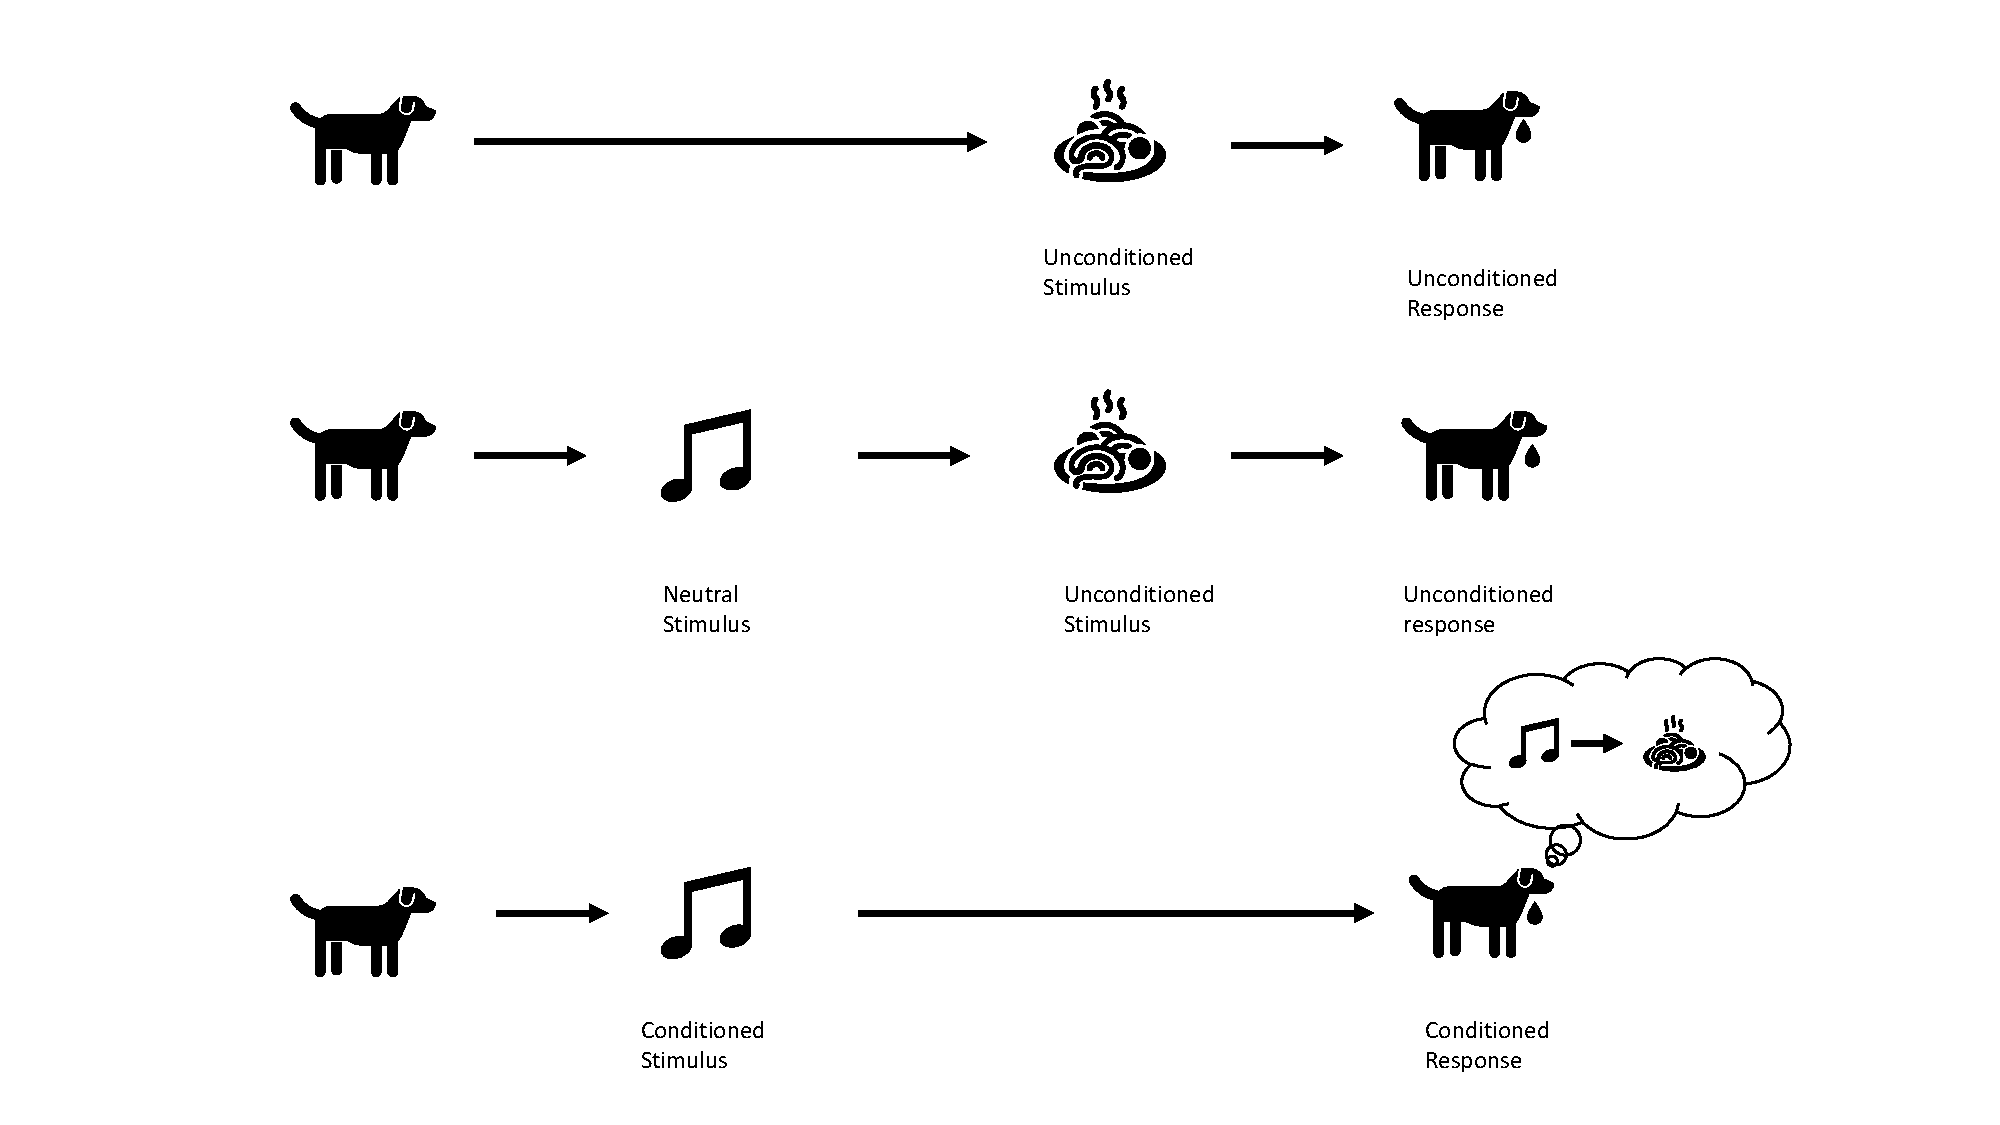
\includegraphics[width=1\textwidth]{Plots/ClassicalConditioning.pdf}
    \caption{Classical Conditioning}
    \label{fig:Classical_Conditioning}
\end{figure}

What have we learned from Pavlov's experiments and what does it have to do with human learning? Through the concept of classical conditioning, we see that it is possible to learn to predict certain events. The dogs learned that the arrival of the caretaker or the sound of the metronome preceded the arrival of food. This is one of the essential features of reinforcement learning: trying to predict future outcomes. %Very clear! Good job!


% \subsubsection{Behaviorism}
% Until now, cats and dogs had a great impact on the view of learning. It ranged from association to predicting future outcomes via presented stimuli. However, these animals are not the only animals influencing the view of learning. Pigeons inspired Skinner in 1963 to develop operant conditioning and with this behaviorism, which will lead us to the last main feature of reinforcement learning (RL): prediction via actions. 

% \citet{skinner1963operant} introduced operant conditioning, the idea of reinforcing behavior through rewards or punishment. Unlike classical conditioning, it focuses on the action and not on the stimuli that is presented. In order to examine his theory, \citet{skinner1963operant} created the Skinner box, which differs from Thorndike's puzzle-boxes in that the goal is not to escape but to obtain food rewards. %In a sense, this is sort if a combination of both Thorndike and Pavlov. Maybe this is a way you could transition to Behaviorism? In a Hegelian sense: Thesis (Pavlov) - Antithesis (Thorndike) --> Aufhebung (Skinner)
% This allowed him to observe animals over a longer period of time and he could indeed conclude that the rats that were put into these boxes learned favourable behavior through interaction with the environment. %Several issues with this sentence. Is length of observation the main advantage of Skinner? I think a different framing would be better. Animals, and then you transition to rats. How was he able to conclude that they learned favorable behavior? Isn't the correct terminology that they were conditioned to behave in such a way that produced rewards? 
% This changed their behavior within the boxes entirely.  %Not sure how this follows logically 
% Skinner continued to examine this phenomenon with various experiments and found he was able to shape the behavior of animals in specific directions. For example in a pigeon experiment, he was able to teach a pigeon to bowl a wooden ball. %Citation
% He did this by reinforcing specific behaviors, which in the end, led to the pigeon learning to pick up the wooden ball and throw it in the right direction. Unlike Thorndike, Skinner concluded that the right actions are learned over the accumulation of random actions that will lead to the correct action. %How is this different from Thorndike? The argument here is unclear

% %At the end of the discussion of each theory, provide the reader with some notions of the limitations and why the problem of learning is not yet solved. 


\subsection{From Classical Conditioning to Prediction Error Learning}
Up until now learning was understood as a passive association between experiences and rewards which could lead to predictions about outcomes. However with the development of computational models, like the Rescorla-Wagner model (RW) \citep{rescorla1972theory}, learning became an active process that is based on a prediction error. This type of learning involves active prediction of the rewards, which are then compared against the true outcome. This prediction error is used to update the previous predictions in order to minimize the error and to improve future behavior. 

%The RW model provided a new approach to learning, by recasting in a more active sense of forming concrete predictions of reward. The model requires the calculation of prediction error (i.e., the difference between expected and actual reward), which requires active predictions of future outcomes. In contrast, the process of learning in classical conditioning is merely a passive association of stimuli and reward. Thus, the RW model provided a new formal mechanism for how learning is not only passively learning associations between actions and outcomes, but rather involves active predictions of rewards. These predictions are then compared against the true outcome, and the magnitude of the error is used to improve future behavior. %I've rewritten these preceeding sentences to be more clear. Consider it as only a guideline
%From the idea of only associating rewards with specific actions to the idea of how trial and error learning is accomplished changed to the idea of predicting the future, observing the presence and updating ones own beliefs in order to minimize the difference between what one calculated and what actually happened in order to predict more accurately the next time and thus improve future performance. %CW: this seems like a rehash of what has already been said, but in less clear terms. 

This concept is similar to the delta-rule \citep{widrow1960adaptive, gluck1988conditioning, yechiam2005comparison}, a learning rule used in machine learning algorithms. The delta rule, also known as the least square method, is used, like the RW, to update previous knowledge based on the prediction error. 
%The delta rule is used in neuronal networks as well as in regression analysis of parameter estimation. 
We can define the delta rule like this: 
\begin{equation}
    E_{t,j}= E_{t-1,j} + \alpha_{t,j}[R_{t,j}-E_{t-1,j}]
\end{equation}
where $E_{t,j}$ describes the predicted reward on a specific trial $t$ and for a specific option $j$. The learning rate $\alpha_{t,j}$ is in an interval between 0 and 1. $R_{t,j}$ denotes the observed reward. In short: the delta rule used the previous prediction and adds the prediction error multiplied by a learning rate to this in order to gain the new prediction. This shows, it uses previous observations and updates these via the prediction error. 
This rule is frequently used as a learning rule in neuronal networks or as a statistical method in data fitting. For example, when fitting data it uses the data itself and the models prediction and then we update the model and its parameters based on the difference between the data and the prediction. The least square method differs in the way that it further penalizes the error by squaring it. Therefore, a greater update is needed to reduce the error. 
%TODO: provide equation
% From \citep{speekenbrink2015uncertainty} we have the following rule: 
% \begin{equation}
%     E_j(t)=E_j(t-1)+ \delta_j(t)\eta[u(t)-E_j(t-1)]
% \end{equation}
% $\eta$ is the learning rule which lies between 0 and 1.  
% u(t) - utility of the reward received on trial t
% $E_j(t)$ expectancies regarding the utility 
% delta 1 or 0 if arm is chosen 

\subsection{A Computational Approach to Reinforcement Learning}
%You need a better stucture for this section. Also, I think you may have some misunderstandings regarding dynamic programming and MDPs. This is totally fine, since you are not expected to be an expert in every field. However, I would try to narrow the focus to what you are comfortable with in order to provide a better discussion. You don't have to cover everything! Just tell a clear and interesting story.
In the history of the reinforcement learning (RL), two kind of RL emerged: human RL, which focuses more on psychological findings and using computational models to understand the behavior, and RL based on dynamic programming, which is set in the field of machine learning and AI. 

Dynamic programming \citep{bellman1960dynamic} was developed by Robert Bellman in the 1950s and is concerned with optimal control \citep{sutton2018reinforcement}. The environment of dynamic programming problems are described as Markov decision process (MDP), which is a discrete stochastic version of the optimal control problem \citep{sutton2018reinforcement}. MDPs can be describes ad sequential decision making processes, which assume the Markov principle: they need a previous state to predict the next state. Actions taken in MDPs influence the rewards (which changes by choosing other options) and also the future states. Solutions are defined as value functions, functions that estimate how good an action is \citep{sutton2018reinforcement}. Dynamical programming concerns itself mostly with optimal value functions like the Bellmann Equation \citep{bellman1960dynamic}. However, these probelms suffer under the so called ``curse of dimensionality''\citep{sutton2018reinforcement}, e.g. the computational complexity grows exponentially with more states. The problem of optimal solution strategies and the curse of dimensionality will be further discussed in \ref{ch:explo}.


% Stochastic optimal control problems, and its solutions like Markov decision processes, are the problems that resemble the problems we considered the most. %Are you saying a MDP is a solution to a stochastic optimal control problem? This isn't true. An MDP is a way to describe the state space relationships by assuming the Markov principle (i.e., only the previous state is necessary for predicting the current state)
% Markov decision processes are a formalization of sequential decision making \citep{sutton2018reinforcement}. This means they can be used to describe problems we have considered before.  
% However, since dynamic programming deals with optimal solution, this as well as Markov decision processes, are computationally expensive and take a long time to be solved. We will consider a specific example of optimal control in the following section. 

\section{Human Reinforcement Learning}

Human reinforcement learning deals with the exploration-exploitation dilemma as its core problem, which is how to balance exploration (e.g looking for a new coffee shop) and exploitation (going to the same coffee shop again). Human reinforcement learning is seen as a field in psychology and cognitive science, which addresses the problem by conducting experiments and modeling human behavior with computational models. 
The dilemma can be investigated with the multi-armed bandit problem, which was first introduced by \cite{thompson1933likelihood} in 1933. It represents a less complex form of the exploration-exploitation dilemma as real life examples. 
   

%I've taken the liberty here to rewrite this paragraph based on some commented out text below, which I thought provides a better introduction than what was currently here. It is far from perfect, but perhaps provides some inspiration for how to write this section
\subsection{Multi-armed Bandit Problem}
The multi-armed bandit problem (MAB) is inspired by slot machines in casinos, which are called one-armed bandits. Each slot machine gives a reward when the lever or arm is pulled. In the MAB problem, you can imagine multiple of these slot machines standing next to each other, where one slot machine represents one arm of the MAB. 
The rewards the slot machines gives out are drawn from underlying probability functions, which are called reward functions. This just means that you do not only get the same reward from each option but there can be a variability in the rewards for each option. To make it more intuitive, think about the coffee example: you do not get the same quality of your coffee every time you buy one in the same shop; the quality can vary. 
%Thus, our coffee example is an instance of a MAB problem. But how can we solve it? 
In a classical experiment using the MAB framework \citep{cohen2007should, daw2006cortical, schulz2017putting}, the decision--maker has a limited amount of decisions (i.e. limited horizon) and the main goal is to achieve the highest possible accumulated reward.
How would you chose a slot machine?
This setup is based on learning from ones own experiences by interacting with the environment, therefore providing a great framework to study the exploration-exploitation dilemma. The MAB will be discussed further in ~\ref{ch:explo}.

%Now what else is there to say about the MAB problem? Provide some examples of important findings, with citations. There are currently some bits that are repeats of the paragraph above, so please make sure it is updated
 %This is somewhat repeated above



%The multi-armed bandit (MAB) problem is inspired by slot machines in casinos (commonly called a one-armed bandit). Each slot machine can produce rewards when the arm is pulled, however the reward distribution is assumed to be unknown. The MAB problem, imagines if you were faced with a row of slot machines, each with different reward distributions, how would you decide which arm to pull? This setup provides a colorful metaphor for a choice problem, where outcomes have to be learned from experience and the goal is to acquire the highest total reward across multiple choices. This provides a very useful framework for studying the exploration-exploitation dilemma because....

 
%CW:This paragraph below didn't do a very good job of illustrating the task to someone unfamiliar with it, so I cut it for now. However, there are good parts that could be reused above
%Bandit problems are types of reinforcement learning problems with the exploration- exploitation dilemma as its core problem. It is an evaluative feedback problem, which means that a response is given about how good the chosen action was. The name and the problem were inspired by slot machines in casinos, which are called one armed bandits. When you pull the lever of such a machine it will give you a reward, if you are unlucky, you won't get any. The bandit problem in reinforcement learning is similarly structured, only that you always get a reward when you choose a lever. The levers are the given options. The most common type of bandit problem is the two armed bandit, which has two options. For example, you can imagine this as two slot machines next to each other or if we look at our coffee shop problem: you have two shops to choose from.
%There are multiple versions of this problem and are all summarized under the term multi-armed or \textit{K}-armed bandit, so you can basically have any number of options available. 



%The name and problem itself was inspired by slot machines in casinos. Those machines produce unknown rewards if you pull their lever. In the bandit problem, each arm of a bandit is inspired by one of those slot machines. Thus, if there is more than one arm, you can imagine as if you would sit in front of more than one of those slot machines and now you are able to decide which lever to pull.
%In this problem, you are faced with choosing between different choices. After each choice, you get a numerical reward as a feedback. Usually, the amount of choices is limited and the main goal is to achieve the highest possible total reward. 
%The simplest version of the multi-armed bandit problem is the two-armed bandit. There only two choices are available. It is commonly used in economics where one of the arm usually gives a steady reward while the other one produces more uncertain rewards, which are drawn from a probability distribution, or reward functions. There are of course, variations where both rewards are drawn from different reward functions.  

%You could also give some intuitions about how the Gittins index works. It transforms the bandit task into a series of optimal stopping problems, thereby providing the right order in which to try out the options and when to stop trying them out any further
\paragraph{Gittins Index}
%One approach to solving the MAB problem is through dynamical programming, which provides a framework for deriving an optimal solution. %CITE papers. When was dynamic programming first applied to RL or for  bandit problem?
\cite{gittins1979bandit} found an optimal solution algorithm for certain versions of the MAB problem, which is referred to as the Gittins Index \citep{gittins1979bandit}. The algroithm does not solve all MAB problems but is 
defined for problems with a finite number of arms (i.e., options), with fixed reward probabilities, and for an \textit{infinite} learning horizon.
This means that only in the limit of infinite time for learning and experimenting, does the Gittins index provide a truly optimal solution. Furthermore, the Gittins Index suffers under the ``curse of dimensionality'´ which means that the complexity of it grows exponentially and is thus not suitable to work with. The curse of dimensionality and the problem of the exponential growth of the problems complexity is further discussed in \ref{ch:explo}. 
%Focus on the infinite time assumption rather than the fixed reward distribution assumption (since we only use fixed rewards)
%This is not moving towards a different argument, of cognitive plausibility. The Gittins index is not truly optimal in finite time, however that alone doesn't necessarily suggest that Humans don't use a Gittins index stategy. Humans also aren't optimal. Rather, you should argue that the computational demands of dyanamic programming are unrealistic.


Humans are capable of solving MAB problems fairly well in real life. Thus we can assume that humans use another way to solve the problem than optimal solutions. But which?   


\section{Exploration--Exploitation dilemma}
The exploration-exploitation dilemma is found in everyday life, if you look for a coffee shop or if you have to make risky decisions \citep{gonzalez2011instance, analytis2019make, schulz2018generalization} or even in small visual tasks \citep{chun1996just}. It is not only applicable to humans, but also to animals, for example: foraging ants that have to find new food sources or keep old ones \citep{cook2013exploration}. 
This shows how extensive the problem is and how many areas it touches. We have already seen two main fields that concern the exploration-exploitation dilemma, human reinforcement learning and reinforcement learning (RL).  

\cite{kaelbling1996reinforcement} describes the exploration--exploitation dilemma as one of the fundamental problems in RL \citep{kaelbling1996reinforcement}.
The dilemma is concerned with finding the right trade-off between exploring to reduce uncertainty and exploiting by choosing the most rewarding option based on the current knowledge of the environment. Exploitation is helpful in order to gain immediate rewards, while exploration is helpful to inform future decisions, through learning which action produce good outcomes. 
Accordingly, the bandit problem is an instance of the exploration-exploitation dilemma and thus also our coffee shop example. 

One possibility to look at this trade-off is by considering strategies how to explore an environment. In which ways can you look at the different coffee shops and reduce your uncertainty about the quality of the coffee? 


\subsection{Exploration Strategies}
%I like this set up with heuristics, but I think you could do a better job of explaining heuristics. I would hope after having attended two summer institutes, you could provide a better account
Full information models, like the Gittins Index are computationally expensive and are not guaranteed to perform well in all circumstances. Full information models take all information into account, this means that they are aware of the underlying reward distribution.
Another approach to explore the environments are heuristics, which do not take all information into account \citep{parpart2018heuristics}, but perform reasonable well and can even outperform optimal solution strategies under realistic scenarios \citep{gigerenzer1996reasoning, gigerenzer1999simple, katsikopoulos2010robust}.
In bounded rationality \citep{simon1956rational} we find the kind of heuristics we are looking for: heuristics which are based on cognitive abilities \citep{gigerenzer2002bounded}. They are especially interesting, because they are used by humans and due to the computational limitation of the human brain do not suffer under the curse of dimensionality.
As \cite{gigerenzer2009homo} pointed out, heuristics are solutions that perform well enough to a certain aspiration level. This means that there is a specific threshold to reach before accepting the solution. As we have seen with the Gittins index, optimal solution strategies are bound to very specific problems and usually need full information about the environment, these information also need to be stable, e.g. they are not allowed to change over time. Therefore, we can assume that most real-world problems are intractable for those kinds of algorithms. Heuristics which do not take all information into account are another approach to solve these problems. Two kinds of heuristics that guide the exploration-exploitation dilemma are widely discussed: random exploration and directed exploration.


\paragraph{Random Exploration}
\begin{figure}
    \centering
    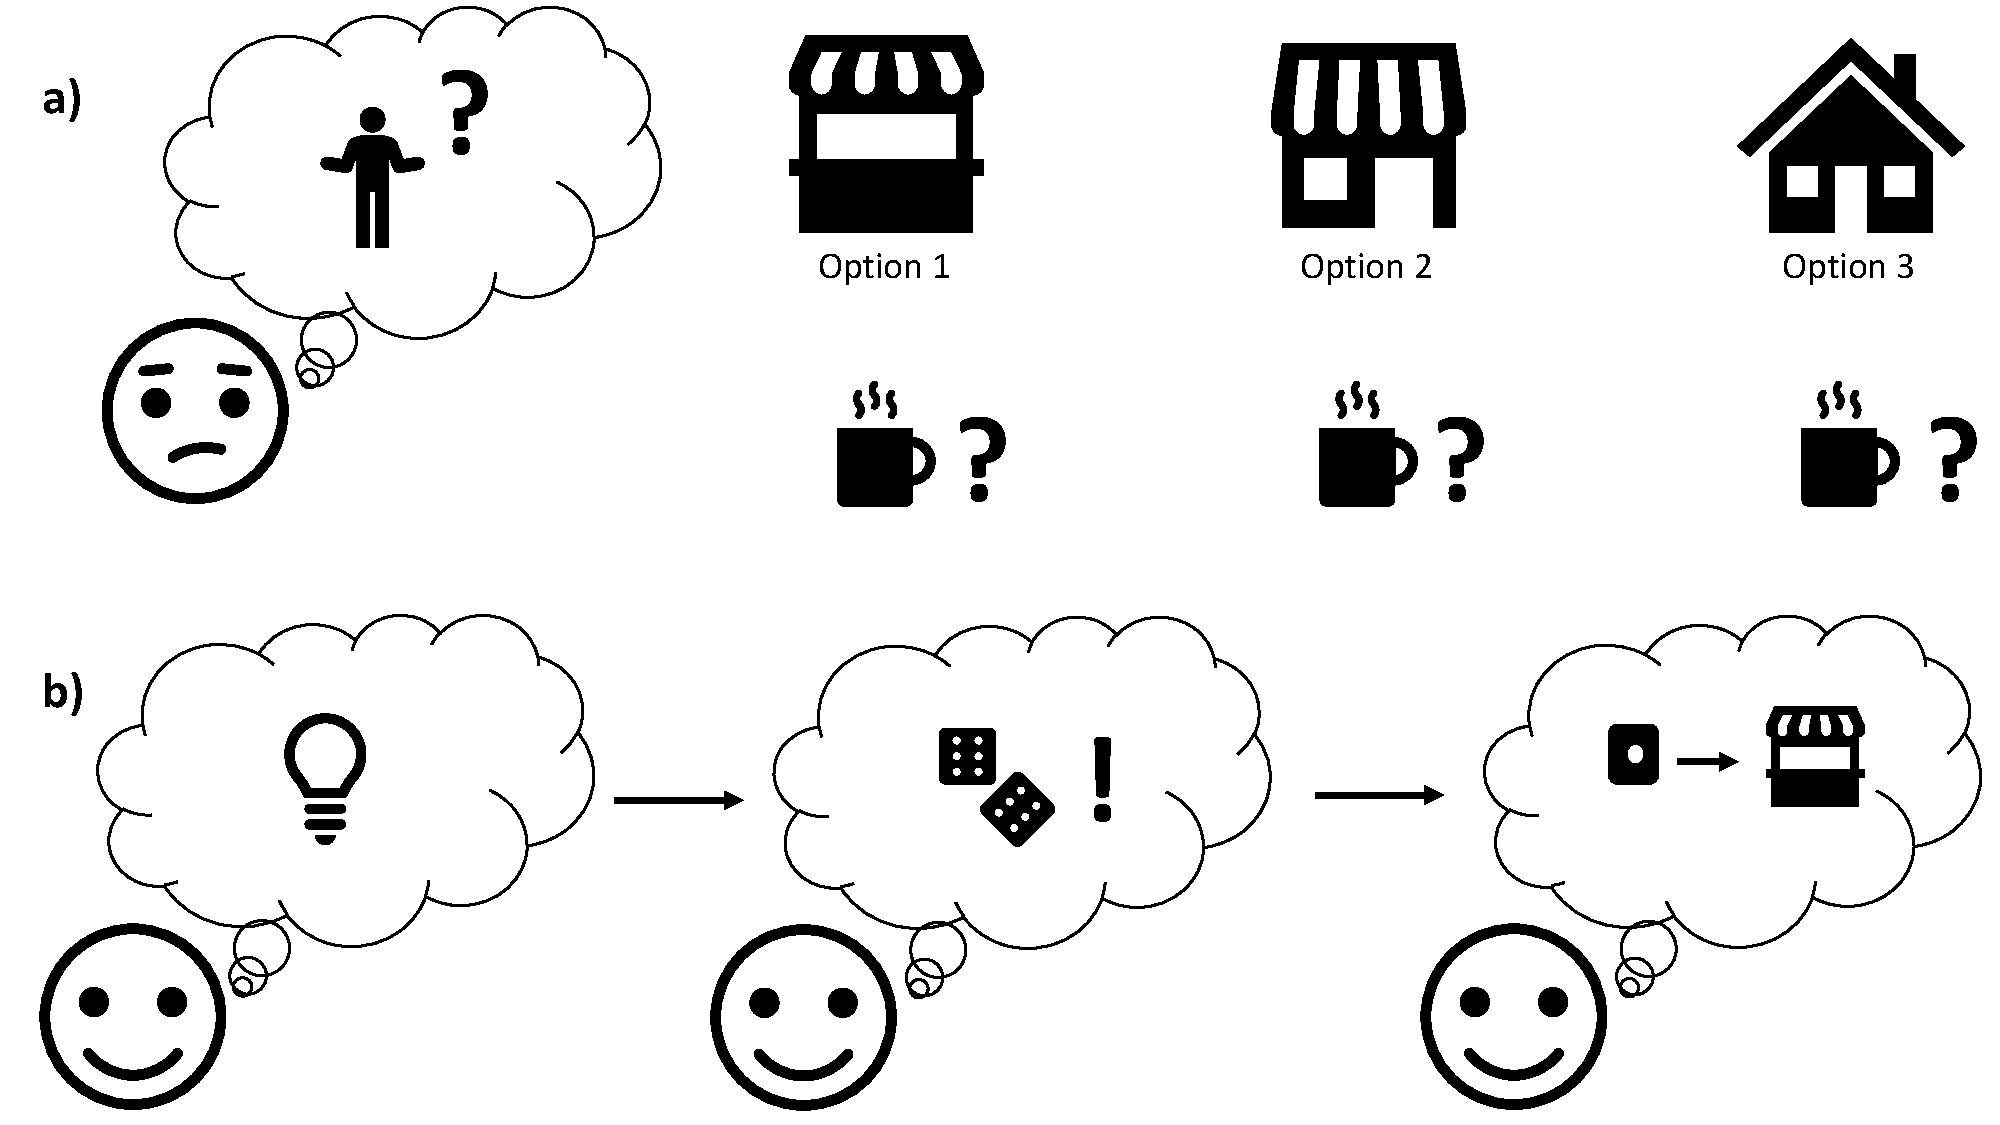
\includegraphics[width=1\textwidth]{Plots/RandomExploration.pdf}
    \caption[Random Exploration]{Random Exploration. In purely random exploration strategies each option has the same probability to be chosen, e.g. an option can be drawn by throwing a dice. If we consider Thompson Sampling, the dice is weighted for the option that has the best outcome, e.g. to always get a six in a dice.}
    \label{fig:RandomExploration}
\end{figure}

%Epsilon-greedy is the purest form of random exploration, but it may be best described along a spectrum
Random exploration is tightly associated with $\epsilon$-greedy algorithms. \cite{wilson2014humans} suggest that they reflect simple heuristics and have less computational cost than directed exploration strategies.  
$\epsilon$-greedy strategies are those kinds of strategies that nearly always preform greedily with only a small probability, $\epsilon$, of sampling randomly \citep[pp.27-28]{sutton2018reinforcement}. A greedy action always chooses the immediate best reward, thus ignoring exploration. In order to adequately explore, the probability of making a completely random selection is included. 

%TODO: provide equation
\begin{equation}
P(c_i) = 
\end{equation}

%Maarten would say thompson sampling is a form of directed exploration, since it uses uncertainty information to guide exploration. Thompson sampling is stochastic, but it isn't really random. Rather, the softmax function with temperature might be a better example
Thompson \citeyear{thompson1933likelihood} sampling is another example of a random exploration strategy.
Thompson sampling is random oriented, which means it randomly draws a value function from the posterior, which is our knowledge about the bandit e.g. the arms and what rewards can be expected. %What does random oriented mean? 
From this random draw it greedily chooses an action, maximizing the immediate reward. In easier terms: we have no complete knowledge of the process of the machine (the bandit), so we randomly assign parameters to it, draw a value function, from which we want to choose an action that will maximize the immediate outcome.

%Don't think this statement is true at all
Random exploration is not as well researched as directed exploration, it is however, studied via model fitting.  
For example, \cite{daw2006cortical} studied a \textit{4}-armed bandit by comparing three different models. One of their models was a random exploration model, the $\epsilon$-greedy model, the other was a weighted belief updating model, which uses the soft-max rule\footnote{options are weighted due to their estimated values}. Their last model was an extended version of their second model with an exploration bonus attached (a directed exploration model). \citeauthor{daw2006cortical} found that the third model with the exploration bonus did not have any evidence from the experimental data. Comparing the remaining two models, the soft-max model had the best fit. %This paragraph is not well developed 

\paragraph{Directed Exploration}
\begin{figure}
    \centering
    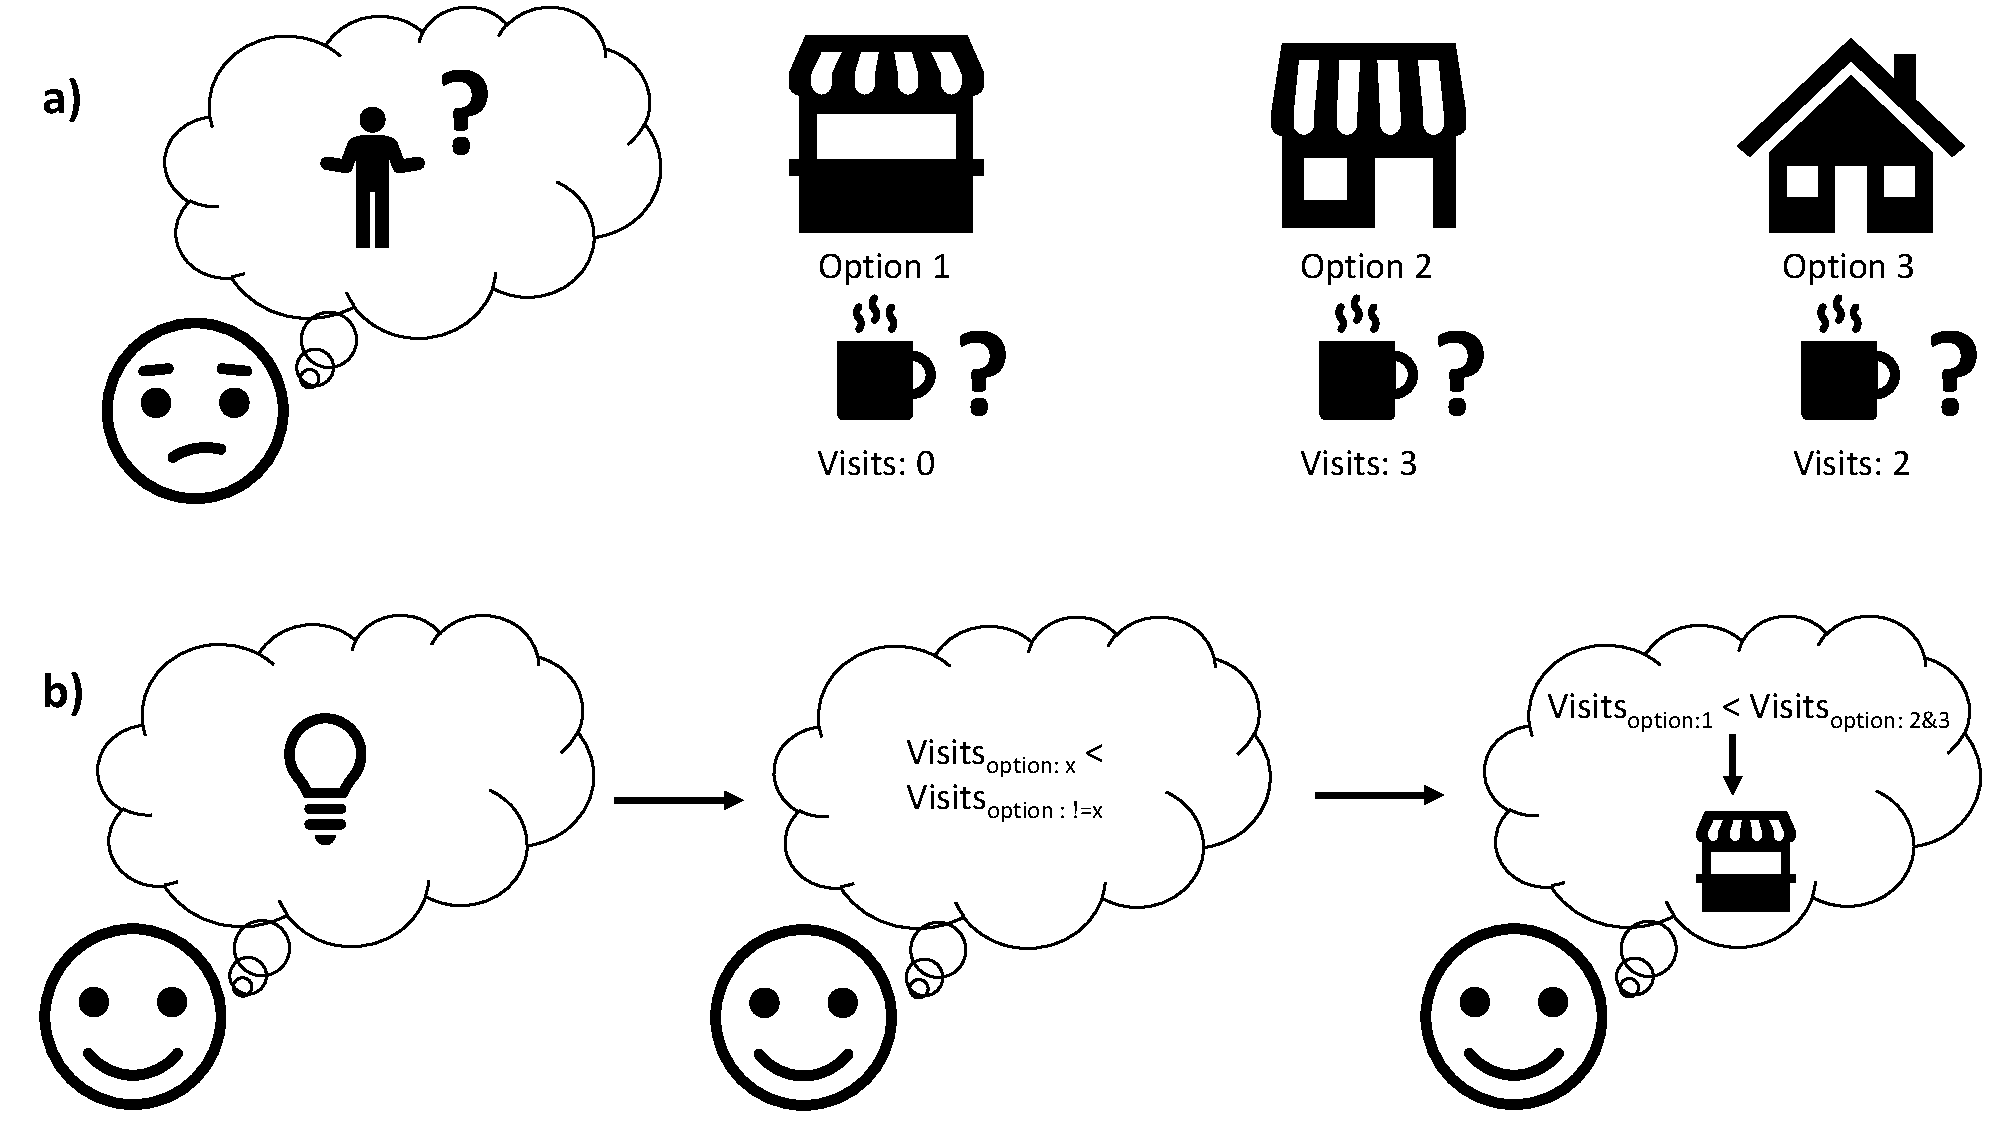
\includegraphics[width=1\textwidth]{Plots/DirectedExploration.pdf}
    \caption[Directed Exploration.]{Directed Exploration. In directed exploration strategies option which we know less about are more likely to be chosen, in order to gain more information andthus reduce uncertainty about the environment.}
    \label{fig:DirectedExploration}
\end{figure}
Directed exploration strategies such as Upper Confidence Bound (UCB) sampling \citep{auer2002finite} are derived from optimal decision making strategies \citep{wilson2014humans}.  %How is UCB derived from optimal decision making strategies?
An exploration bonus is the main component of directed exploration behavior. The bonus leads to weighted exploration, this means that new options are not randomly selected but are encouraged by probabilities concerning their uncertainty. There has been evidence against the use of exploration bonuses in humans \citep{daw2006cortical}. However, more recently there has been more evidence found for the use of this strategy \citep{wu2017mapping, wu2018connecting, wu2018exploration, schulz2018searching, wilson2014humans, gershman2018deconstructing,knox2012nature, steyvers2009bayesian, }.    
\cite{wilson2014humans} assume that there are two main reasons why some studies did not find any exploration bonus. Firstly, direct exploration might be difficult to identify due to a confound between information and reward. They assume that the gained information is confounded with the reward the option yielded, which makes it difficult to identify directed exploration. 
Secondly, they assume that there is an information--ambiguity interaction. In other words: the more information you have about an option, the more it is ambiguous. This would mean, that participants that avoid ambiguity avoid information seeking and prefer exploiting their current knowledge.


Unlike Thompson sampling, UCB sampling \citep{auer2002finite} does not use immediate probabilities to decide which action to use, rather it works in the way that it uses an uncertainty bonus \citep{srinivas2009gaussian}. This basically means that more uncertain options (those you know less about) get a bonus, thus their probability of being picked is higher. This corresponds to the idea, that you accumulate the most information in order to exploit these information later.

%This section provides much needed citations of relevant literature, but it is not well organized. You always start off each paragrap with a \cite{}, but you should be oganizing your writing based on ideas, rather than on citations. Citations offer support and context for your ideas. You need to structure your writing such that you make an argument
\subsection{Current Theories}
The exploration--exploitation dilemma can be described with examples of choice problems, e.g., finding a new favourite coffee shop in a town you recently moved to and in a more scientific way with the bandit problem. %The coffee shop problem is a bandit problem. Not sure I understand your point here
How to solve these problems is not well understood. Optimal solutions have constraints that are nearly impossible to obtain. There are currently two main strategies upon which humans solve these problems, random and directed exploration.  

The first option is exploring an environment only by chance, which is called random exploration. Thompson sampling is an example of random exploration.
The second option is directed exploration, where sampling from more uncertain option is encouraged by adding an uncertainty bonus. The UCB is an instance of this exploration strategy.

\cite{wilson2014humans} investigated the effect of the horizon on those two strategies in order to understand how humans use these strategies or if they use them at all. Their carefully designed experiment allowed to distinguish between both kinds of strategies, due to the assumption that a varying horizon influences the way of information seeking and can even produce decision noise. Therefore, they were able to conclude that both strategies are indeed used and vary depending on the horizon. Given the opportunity to explore more e.g. having a higher horizon, participants rather used a directed exploration strategy, while under a smaller horizon random exploration was used.
In alignment to this finding \cite{gershman2018deconstructing} proposed that humans use a mixture of both exploration strategies, thus promoting a hybrid model of the UCB and Thompson sampling. He concluded that under relative uncertainty\footnote{the relative uncertainty between the option} there was a faster response time, which is consistent with the UCB. Furthermore, under absolute uncertainty\footnote{the overall uncertainty} there was a slower response time, which indicated the Thompson sampling \cite{gershman2018uncertainty}.

\cite{zajkowski2017causal} found a distinction in brain activity for both exploration strategies. In their trans magnetic stimulation experiment, using the same paradigm as \cite{wilson2014humans} found that when inhibiting the right frontopolar cortex, there was a negative influence on the use of directed exploration. It had, however, no effect on random exploration.

If we consider Marr's (\citeyear{marr1976understanding}) levels of explanation , we can argue that exploration strategies would fall into the first level: The computational level, which is supposed to tell us what a system is doing, in our case, which action is chosen. The next step would be to take a look at the second level: The process level. This deals with how one actually ends up making a decision and how the processes behind it work. In other words: How are the decisions made and which processes are guiding this decision?  %This is a very important paragraph but it has gotten buried

\cite{gottlieb2018towards} suggest that learning is governed by curiosity. They assume that animals and humans have intrinsic motivations that value specific types of information gain more than others, which are independent of gaining rewards. This kind of behavior can be studied under active sampling tasks, which are variations of the bandit problem. In order to actually see this phenomenon it is important that the agents is allowed to freely choose which stimuli (or button or source of information) it wants to explore\footnote{in plain information gain tasks, the same behavior can also be seen, suggesting there is an intrinsic motivation to gain information}, before it has to chose an action. 
Considering signal detection theory, or evidence accumulation theories\footnote{the agent has uncertainty about states in the environment and has some control over how much information it sample to reduce this uncertainty} like the drift diffusion model, \cite{gottlieb2018towards} notes that these theories assume that the agent has some knowledge about how to identify relevant cues, without taking into consideration how the agents determines which cue is relevant. 
Furthermore, curiosity is linked to memory \citep{gruber2014states, kang2009wick} and attention \citep{jepma2012neural}, which are important factors in learning.


\cite{collins2012much} studied the relation of working memory and reinforcement learning. By creating a task that allowed to separate working memory specific effects on learning, they were able to set up a new computational model, that was able to better estimate single reinforcement processes. This model is composed of two smaller models one model free reinforcement learning model, which represent slow and cumulative learning, and a second model which represent the working memory and is fast but with limited capacity. In a study in 2014, they were able to test their model on data gathered by schizophrenic patients \citep{collins2014working}, which are know to perform poorly in reinforcement learning tasks. Due to fitting the data to the model, they were able to discover that the impairment for reinforcement learning were governed by deficits in working memory that effects reinforcement learning. 


As we have seen in the passages above from experimental behavior, we can draw conclusion about the process level from Marr's level hypothesis, which is how is the process working. Thus the remaining question is, how and what process governs random and directed exploration. 

\section{Motivation and hypotheses}
Learning by interacting with the environment was first studied in animal learning research [cite thorndike, pavlov], and then developed into the field of reinforcement learning [cite Sutton]. Starting from theories of learning as a passive association of stimuli and reward [CITE], theories developed into more new conceptions requring actively making predictions about the world, and then updating based on the magnitude of the prediction error \citep{rescorla1972theory}. 

The exploration-exploitation dilemma is a central problem in the field of reinforcement learning, which focuses on the trade-off between exploring (reducing uncertainty about the environment) and exploiting (gaining rewards). In particular, the multi-armed bandit (MAB) framework is used to investigate this dilemma. Optimal strategies such as the Gittins Index are poorly suited in real world scenarios, because it assumes an infinite horizon and a stationary environment, both are criterion that are not in line with the real world, as there is a constantly changing environment and there can not be an infinite horizon. %I would remove the focus on stationary environment, since we also use a stationary environment. Rather, focus on the infinite horizon
However, heuristics can perform reasonable well and sometimes outperform optimal decision strategies. Heuristics can be used as exploration strategies in the bandit problem. %These heuristics are combined with psychologically inspired learning models
As we have seen, humans use two kinds of exploration strategies, random and directed exploration, in order to solve the exploration-exploitation dilemma tasks like the bandit problem. %You haven't shown that it is the case yet
These two heuristics can be formalized in the Thompson sampling for random exploration and the Upper Confidence Bound (UCB) for directed exploration. Both strategies are governed by uncertainty, but in different ways. Thompson sampling is governed by relative uncertainty while the UCB is governed by absolute uncertainty.

In order to understand the process managing these decision strategies, and thus gain insight into the cognitive processes underlying human learning, we applied time pressure onto a four armed bandit task. 
By manipulating the decision time, we induce computational limitations, which reduce the ability to sample from memory and accumulate evidence. This provides insight into the underlying processes that manages random and directed exploration, whether people use a combination of both or switch between them. 

\newpage




%\end{document}